\chapter{Interactive Object Recognition}
\label{chapter:Object Recognition}

\section{Challenges}
As suggested in \ref{chapter:Introduction} in feature-matching-based object recognition systems we encounter a lot of difficulties that mainly correspond to view-point-variance of the features as well as lighting conditions. In order to prove that hypothesis we implemented an object recognition system that extracts the features in the database and live images and matches them together. Based on the number of matches the system can detect which object is being seen in the live image.

\subsection{Lighting Conditions}

During our experiments we noticed that a lot features were flickering even though we did not change position of any object in the image. After investigating this issue we came to the conclusion that it is mainly caused by lighting issues that feature detector cannot find the same feature in two consecutive frames. We examined that by searching for the features and then matching them against the live image. We saved two patches: once where the feature was found, and the second one where it was not found. Fig. \ref{fig:patches} depicts above described results.

Looking at the difference image it can be clearly seen that there was a significant change in lighting even though we did not change anything. Corner detector did not find the correct feature in the live image simply because this image looks differently which is caused by the change of lighting conditions.

\begin{figure}
%\centering

{
\includegraphics[width=1\columnwidth]{figures/patches.png}}

\caption{Difference between two pairs of images taken without taking any action in between. The first patch of the pair shows the area in the database image where the feature was found. The second patch shows the area in the live image where the corresponding match was found. After subtracting one pair from another and multiplying the difference by the factor of 10, the significant difference in live image patch is visible. There is no difference in the database image patch because it is the same patch for both pairs.  It indicates the influence that lighting has on the image. }
\label{fig:patches}
\end{figure}

\begin{figure}
%\centering
    \begin{tabular}{c}
 

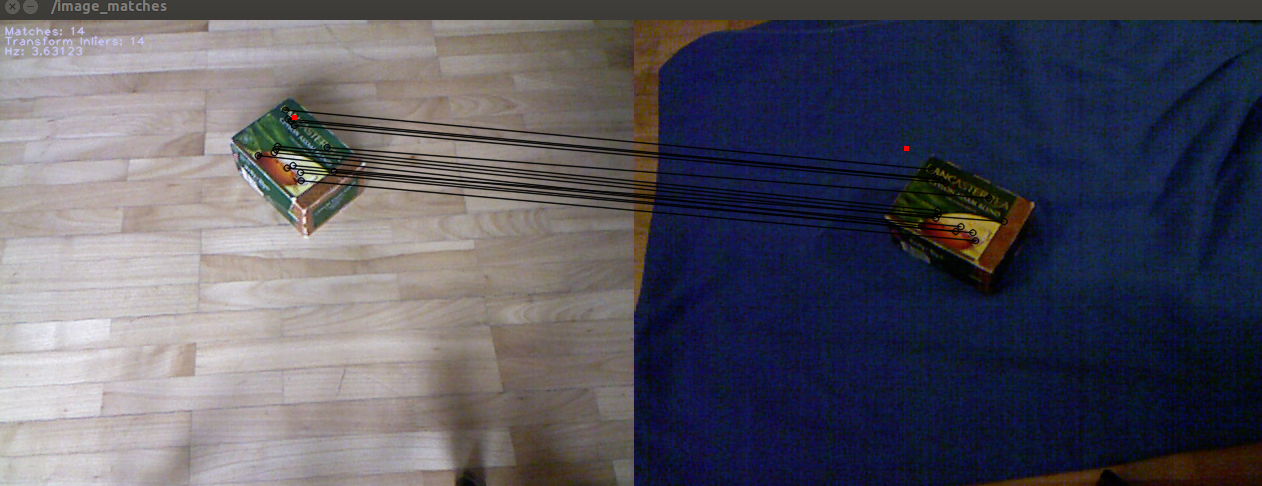
\includegraphics[width=0.7\columnwidth]{figures/sift-gpu-no-rotation.png}\\
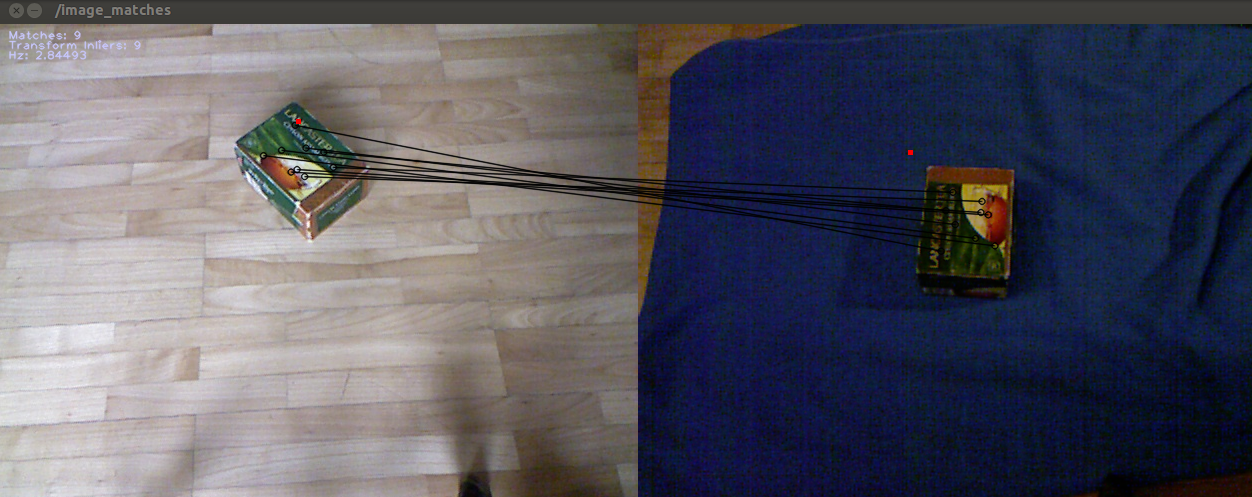
\includegraphics[width=0.7\columnwidth]{figures/siftgpu-rotation.png}\\
    \end{tabular}


\caption{Comparison of two pairs of images using SIFT detector and SIFT descriptor. The upper image shows the object in the original pose whereas the lower shows the rotated object. It can be noticed that number of feature matches significantly decreases if the object is rotated. }
\label{fig:sift-features}
\end{figure}

\begin{figure}
%\centering
    \begin{tabular}{c}
 

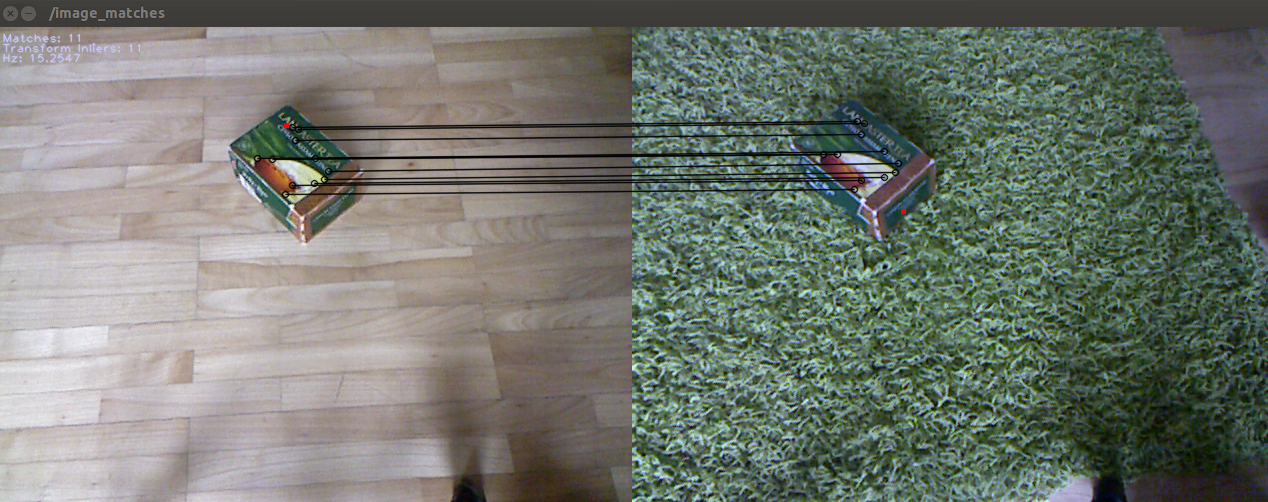
\includegraphics[width=0.7\columnwidth]{figures/freak-no-rotation.png}\\
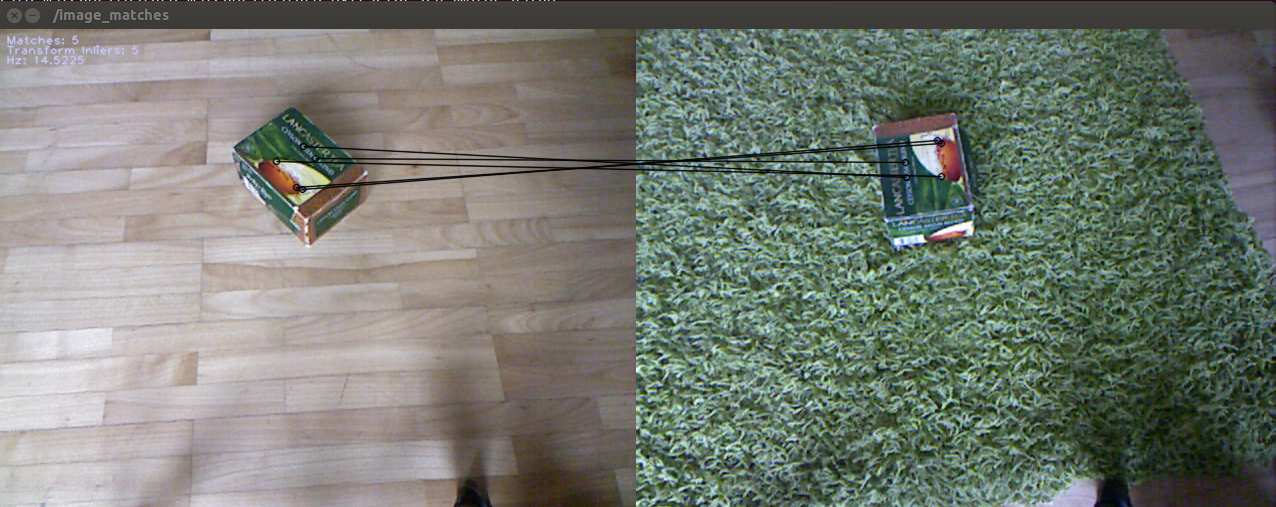
\includegraphics[width=0.7\columnwidth]{figures/freak-rotation.png}\\
    \end{tabular}


\caption{Comparison of two pairs of images using FAST detector and FREAK descriptor. The upper image shows the object in the original pose whereas the lower shows the rotated object. It can be noticed that number of feature matches significantly decreases if the object is rotated. }
\label{fig:freak-features}
\end{figure}

\begin{figure}
%\centering
    \begin{tabular}{c}
 

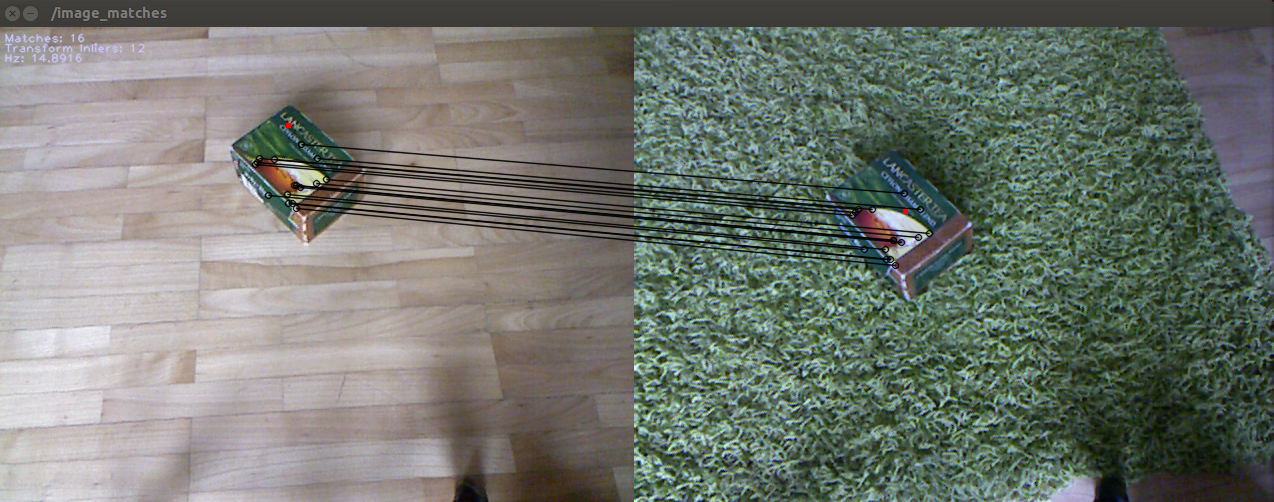
\includegraphics[width=0.7\columnwidth]{figures/brief-no-rotation.png}\\
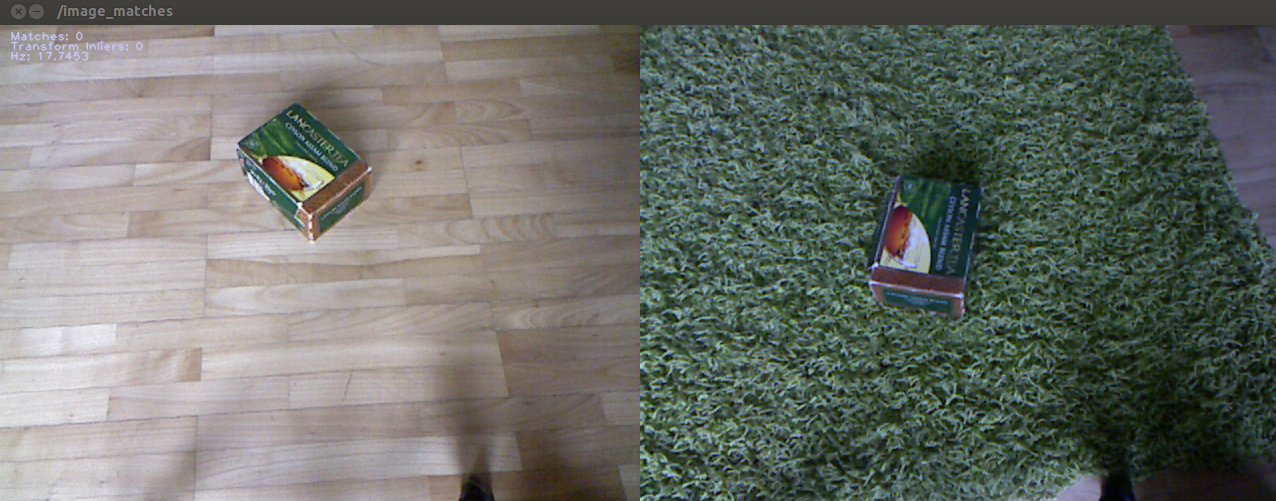
\includegraphics[width=0.7\columnwidth]{figures/brief-rotation.png}\\
    \end{tabular}


\caption{Comparison of two pairs of images using FAST detector and BRIEF descriptor. The upper image shows the object in the original pose whereas the lower shows the rotated object. It can be noticed that number of feature matches significantly decreases if the object is rotated. }
\label{fig:brief-features}
\end{figure}


\subsection{View-point Variance}

In order to show the problem of view-point variance of the feature descriptors we compared two live images of the same object - one in the same pose as it is in the database and the other one when the object is rotated around Z axis. We tested those pairs with three different detectors and descriptors to ensure that the problem is not connected to a particular detector-descriptor pair. The results are depicted in Fig. \ref{fig:sift-features},\ref{fig:freak-features} and \ref{fig:brief-features}.

Looking at Fig. \ref{fig:sift-features},\ref{fig:freak-features} and \ref{fig:brief-features} it is noticeable that the number of matches significantly decreases when the object is rotated. Even with the most rotationally and view-point invariant feature detector-descriptor pair - SIFT - drop of the features equals 35$\%$.



\section{Approach}

Following our idea to leverage robot's capabilities in order to improve perception we employ interaction with object as a tool that is likely to partially solve the latter of above mentioned challenges. In our approach we use the rotational movement of the object in order to eliminate the influence of view-point variance of features.

\begin{figure}
%\centering 

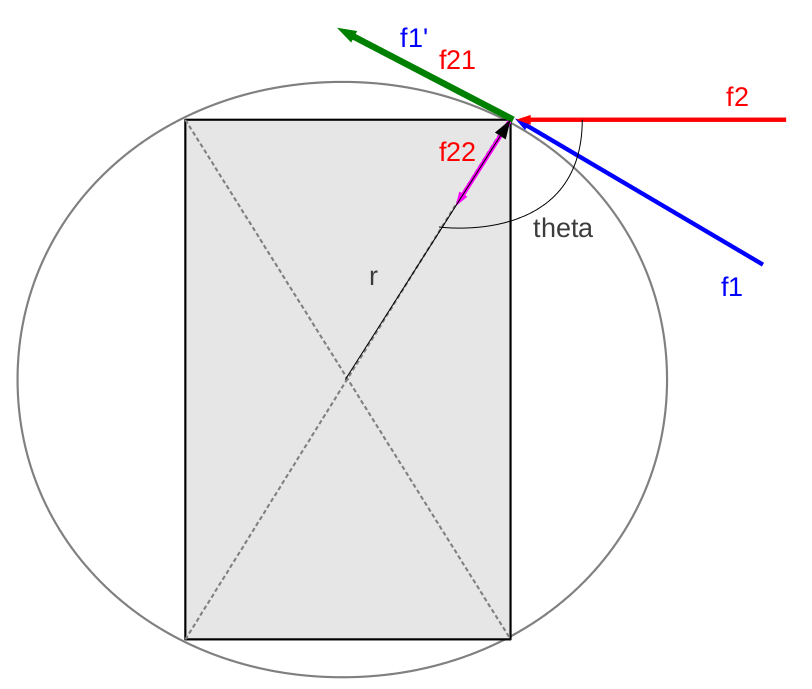
\includegraphics[width=0.5\columnwidth]{figures/rectangle-angle.png}\\


\caption{Object under the influence of two forces. F1 shows the tangential push that will result it in only rotational movement, hence in the force - f1\' tangential to a circle exscribed on the object. F2 shows the proposed pushing strategy - perpendicular to the longer egde. This push results in two forces - f21 tangential coefficient responsible for rotation and f22 - translational coefficient. In this case object will not only rotate but also translate in the direction of f22 force.  }
\label{fig:angles-rectangle}
\end{figure}


\begin{figure}
%\centering
 

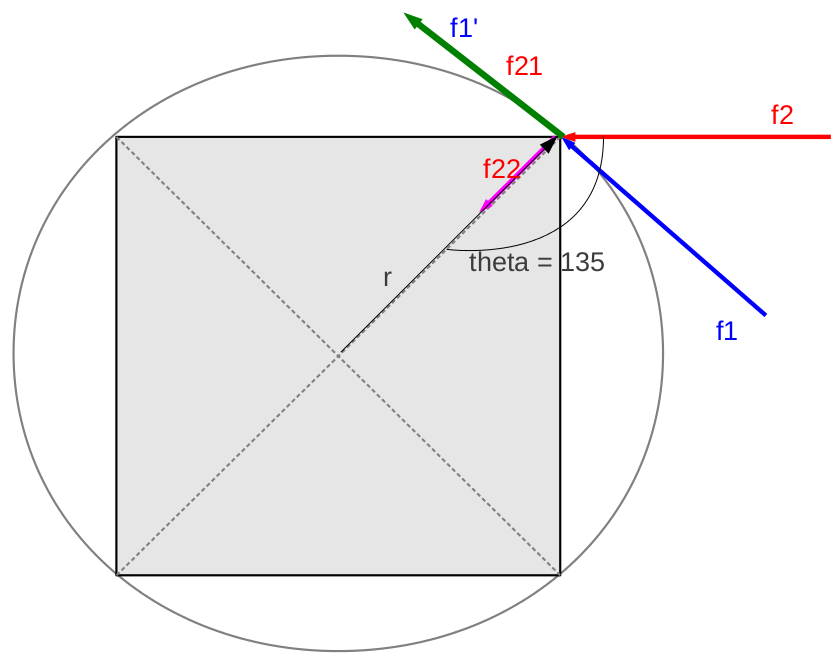
\includegraphics[width=0.5\columnwidth]{figures/square-angle.png}


\caption{Extreme example of energy loss of the proposed pushing strategy on the squared object. Theta is in this case maximal and equals 135 degrees. It results in a energy loss of 30\%  }
\label{fig:angles-square}
\end{figure}

\begin{figure}
%\centering 

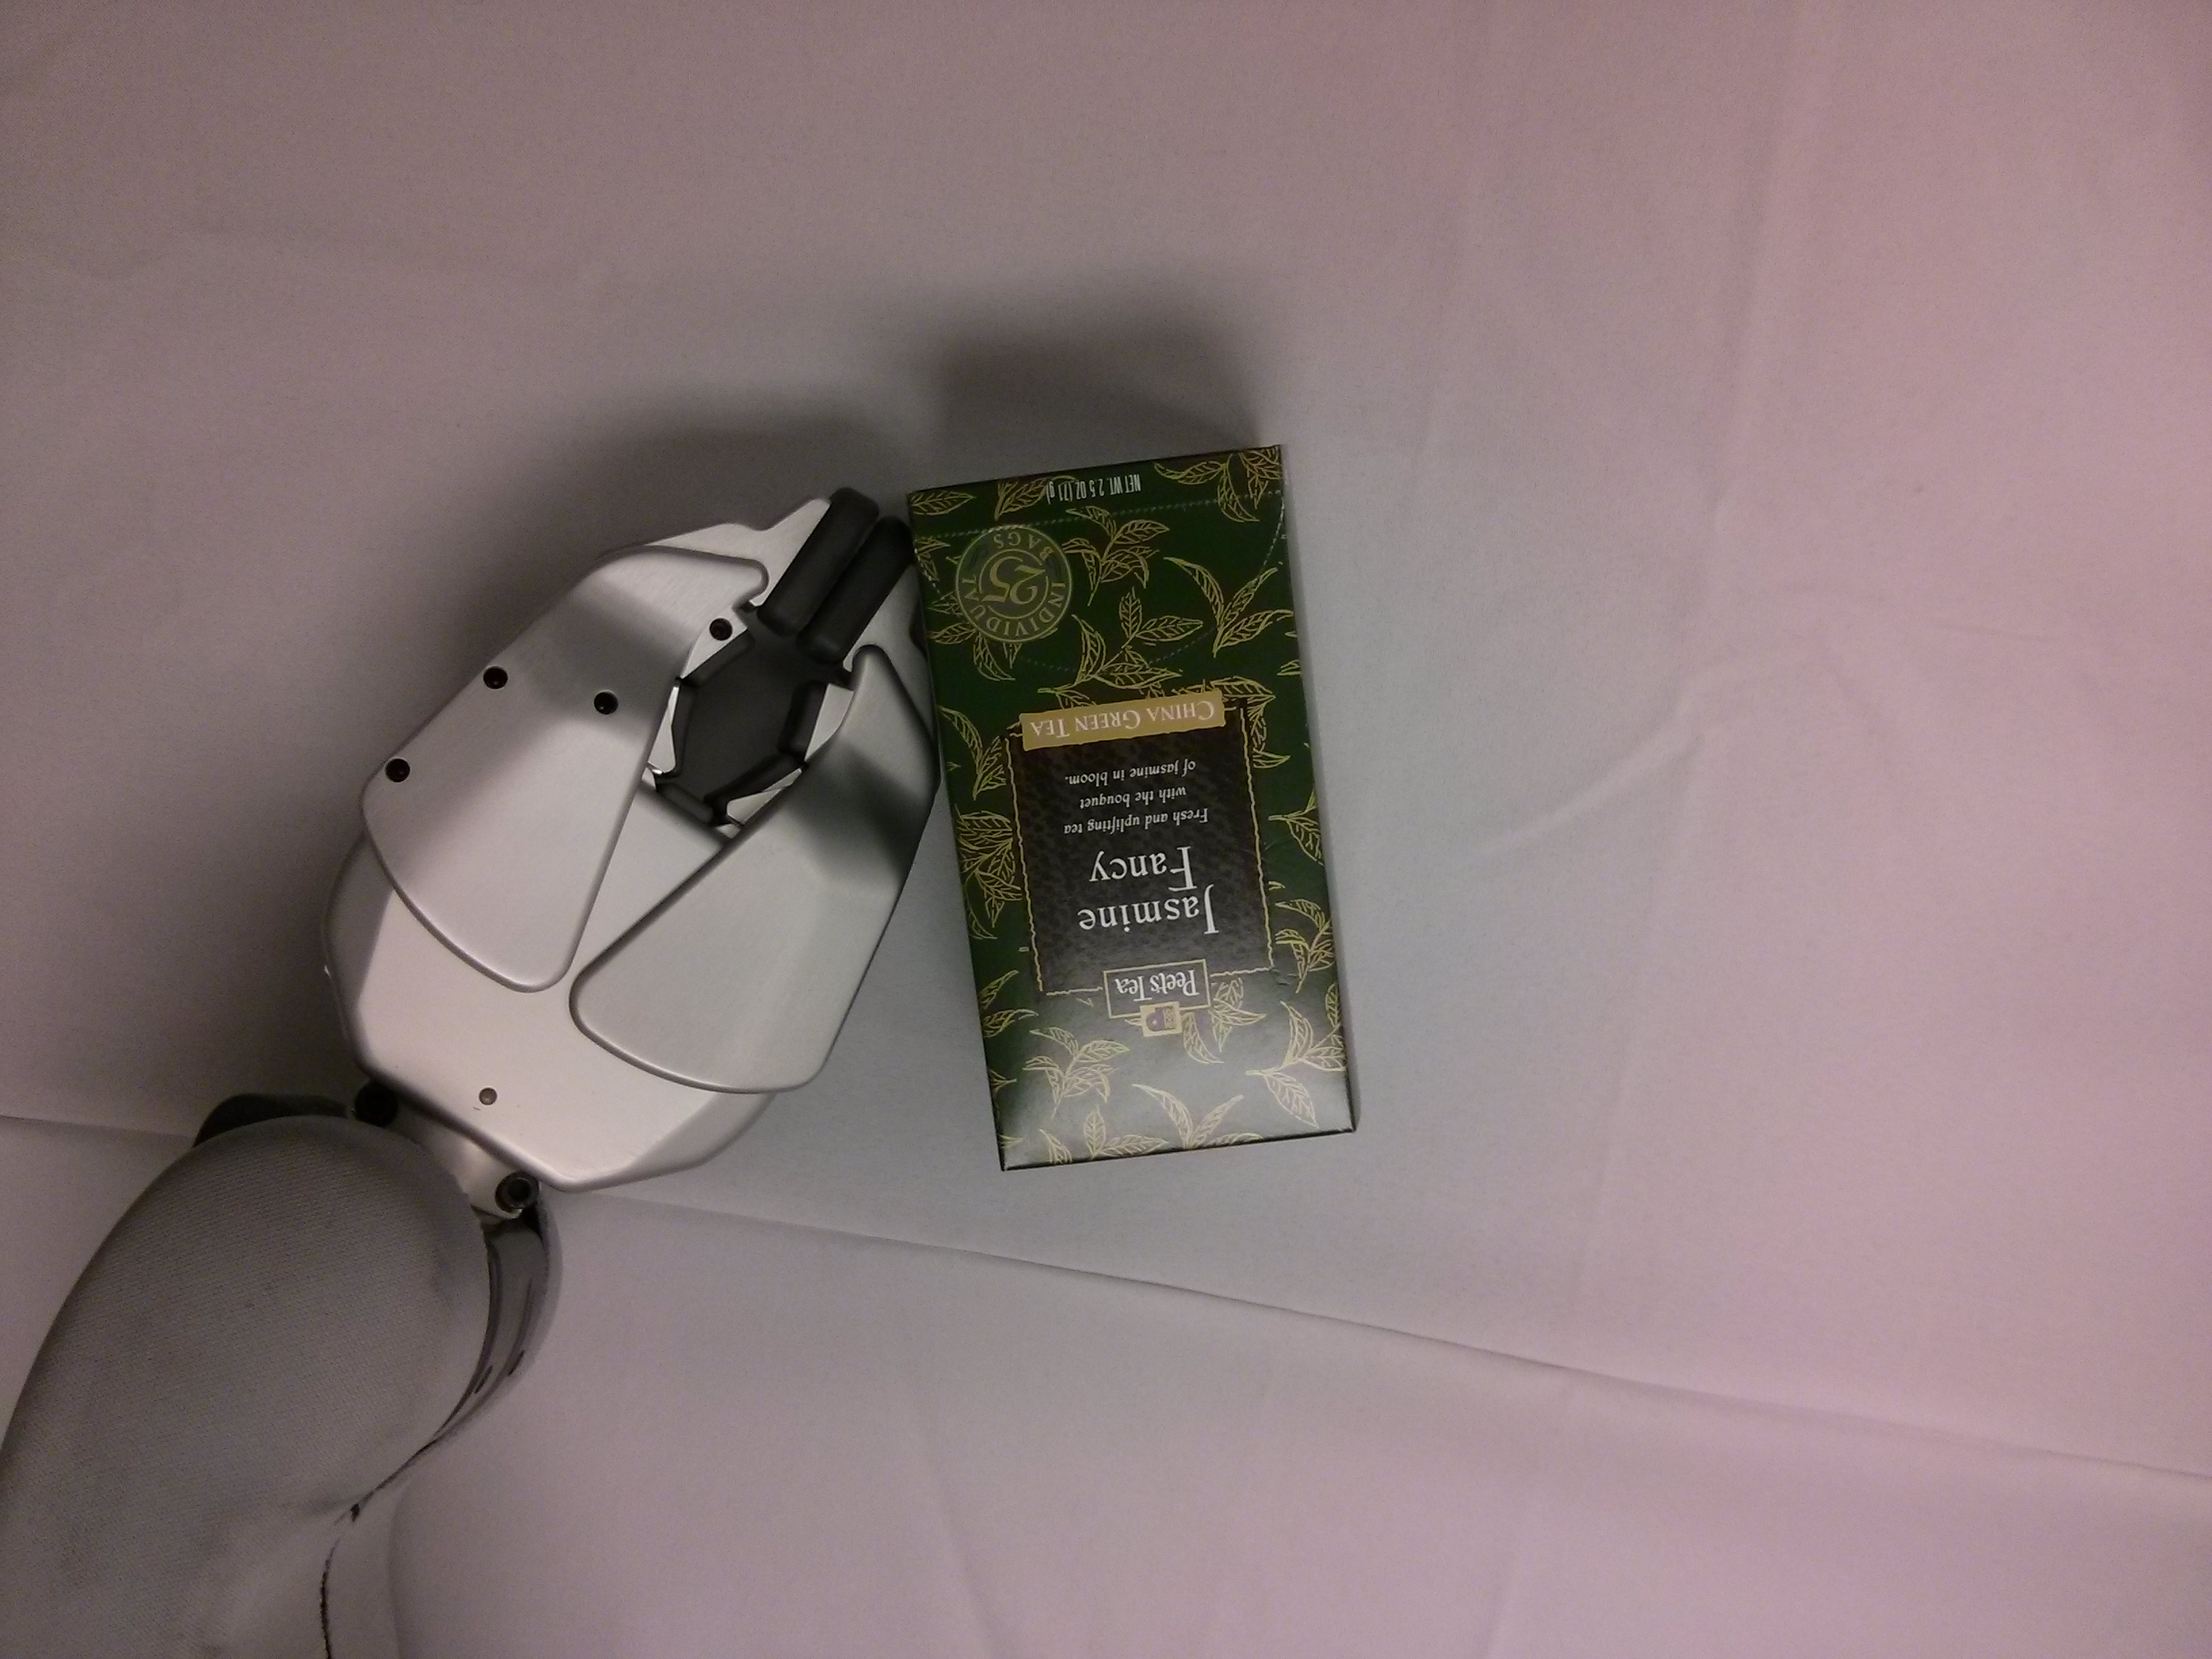
\includegraphics[width=0.4\columnwidth]{figures/peets-tangential.jpg}\\
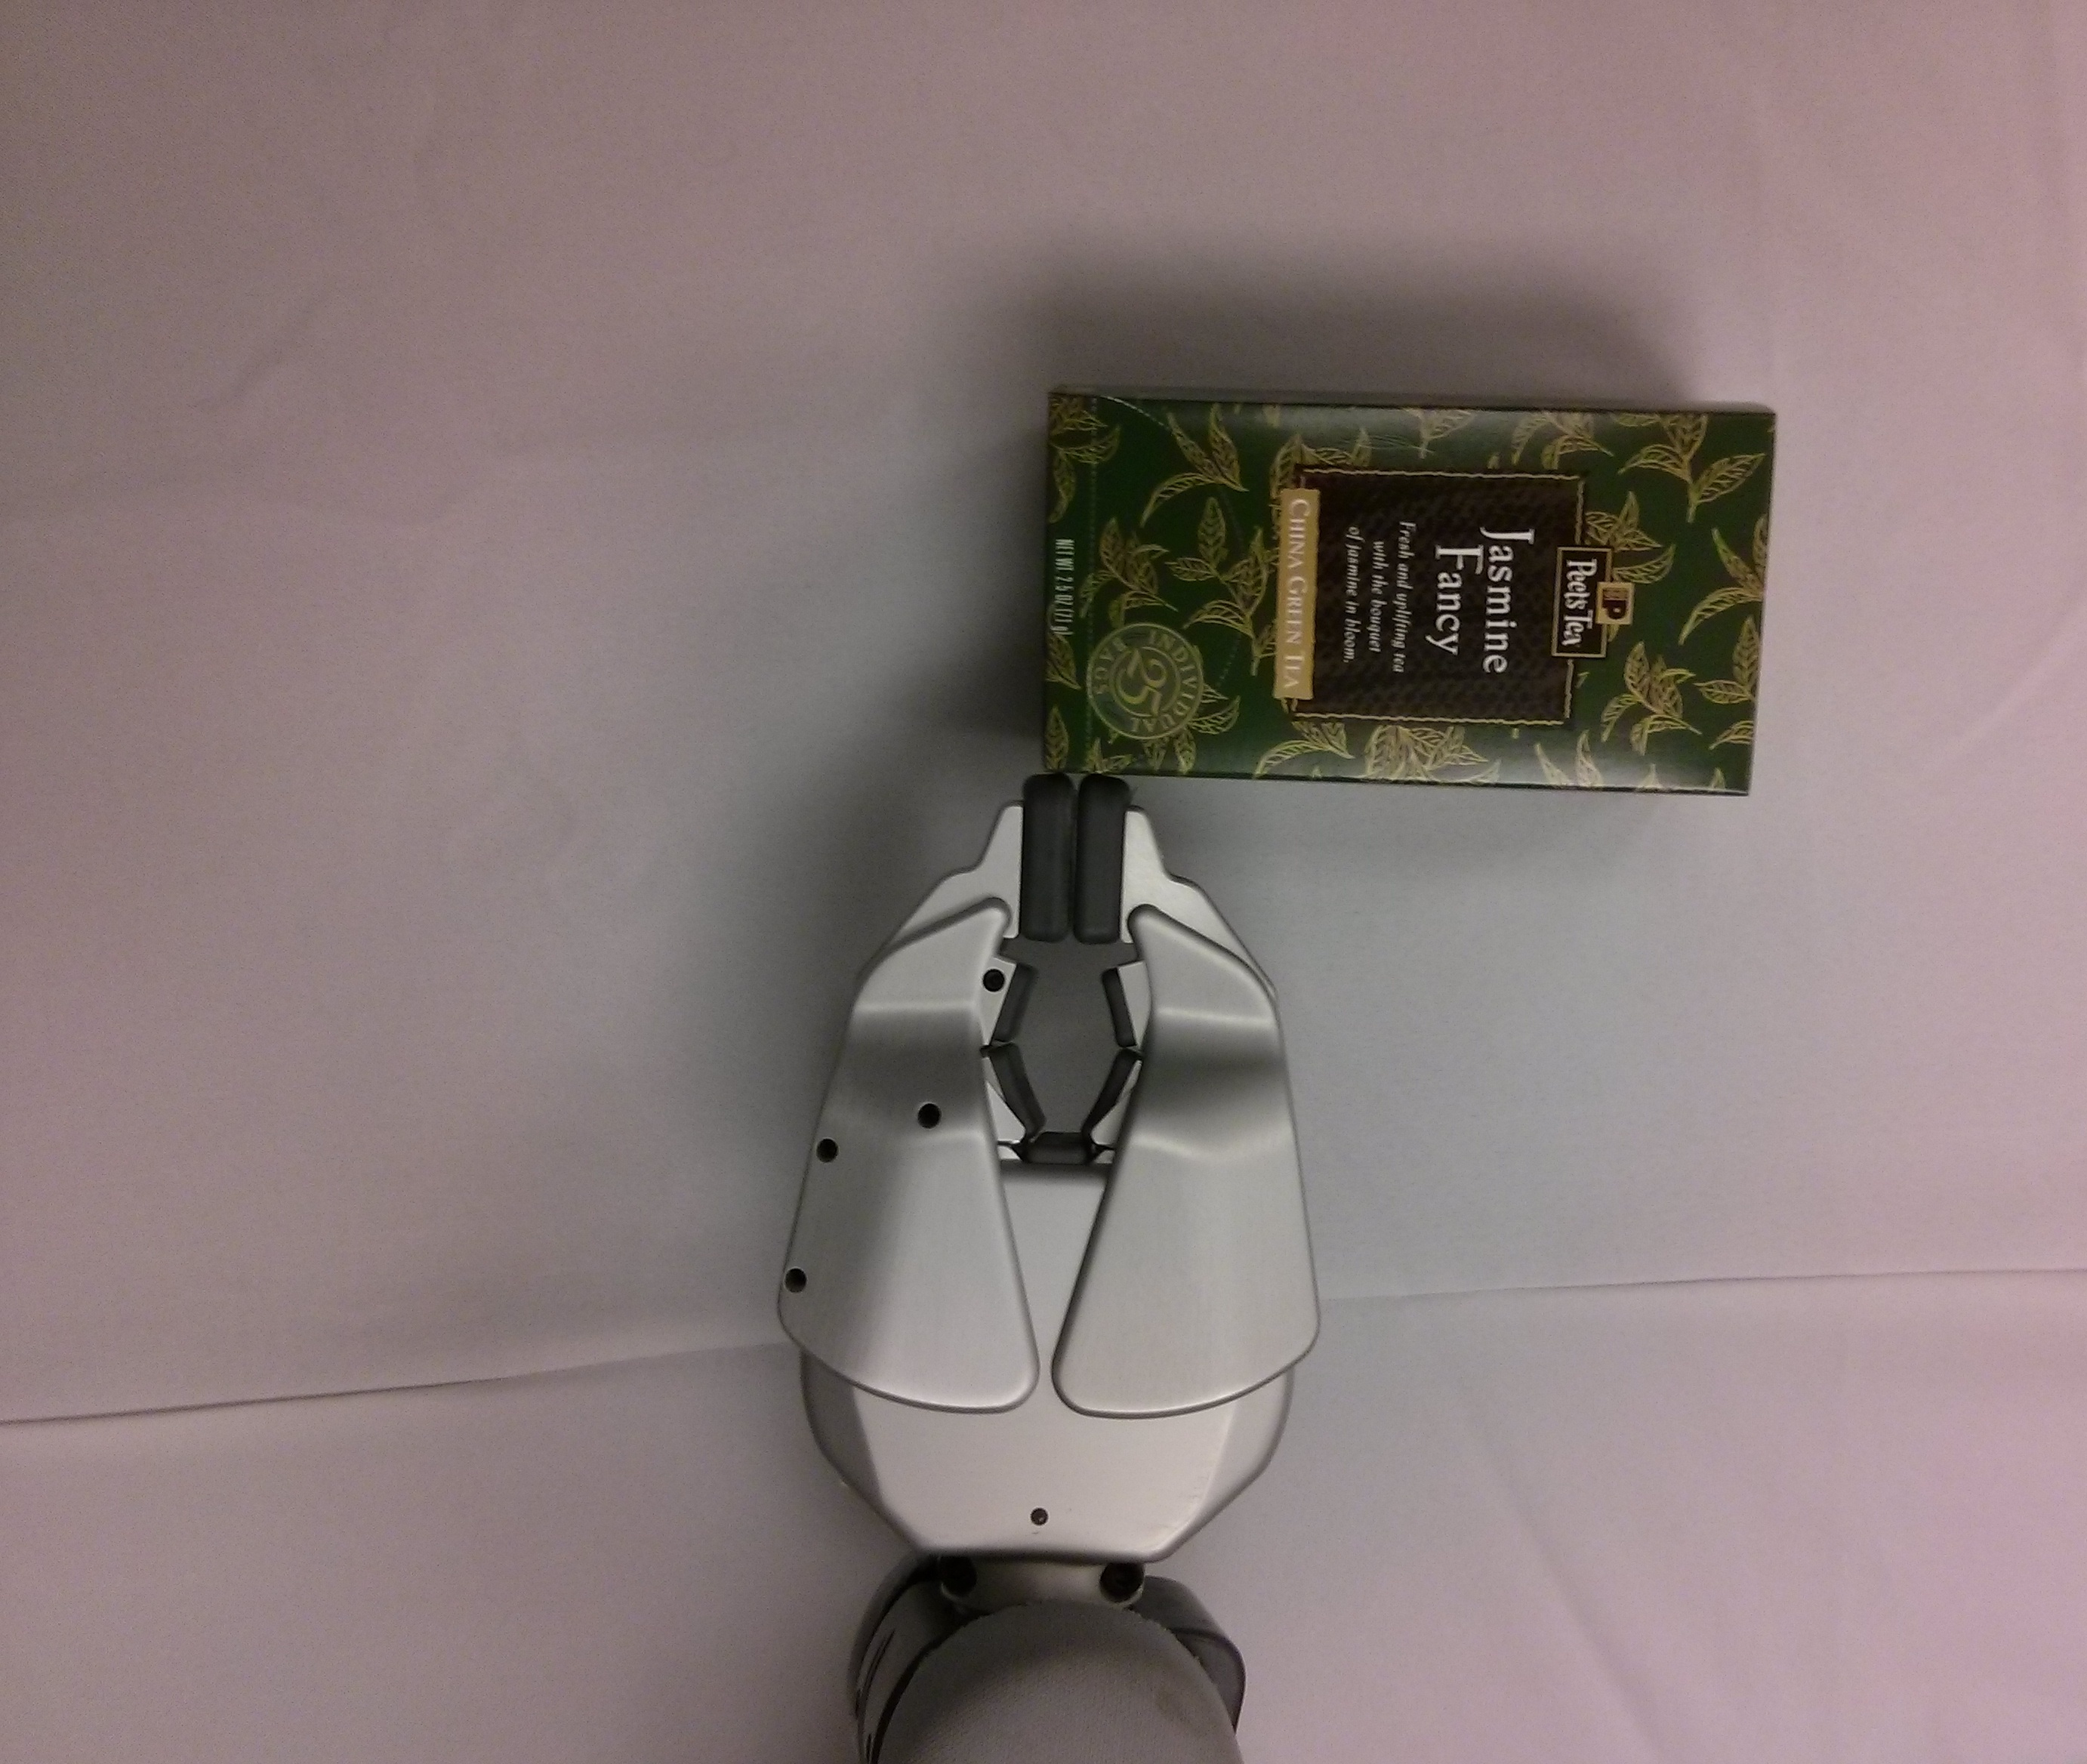
\includegraphics[width=0.4\columnwidth]{figures/peets-perpendicular.jpg}\\


\caption{Upper row - example of tangential push. Lower row - example of perpendicular push.}
\label{fig:tangential-example}
\end{figure}


\subsection{Rotation of Objects}
In order for a robot to rotate an object efficiently that is such that the push results in only rotational kinematic energy it is required to maximize the the torgue that acts on the object. As shown in Eq \ref{eq:max-torque} the maximum torgue can be obtained with the biggest $r$ component that the force is acting on and with $sin(\theta) = 1$.

Maximizing $r$ component results in the point that the furthest from the center of mass of the object. Since we assume uniform distribution of mass, the center of mass of the object is in its geometrical center. Hence the best push point to rotate the box-like object is at the corner which is the furthest point from the center of the rectangle.

In order to fulfill the second constraint - $sin(\theta) = 1$ on the box-like object $\theta = 90 degrees$ which results in tangential push as depicted in Fig. \ref{fig:angles-rectangle} - force f1. However, due to geometrical contraints of the robot's gripper it is difficult to execute tangential push. The upper row of Fig. \ref{fig:tangential-example} shows the box-like object with the robot's gripper in the pose for the tangential push. It can be noticed that due to the size of the gripper the actual contact point between the gripper and the object is not at the corner. The other problem that occurs in this kind of push is that the gripper is likely to slip off the object while pushing.

Because of the above mentioned reasons we came up with a push perpendicular to the longer edge of the object. This push is easy to execute with the robot's gripper while still being able to result in rotational movement of the object. The lower row of Fig. \ref{fig:tangential-example} shows the resulting robot's gripper position related to the object. However, in this case the push is not optimal in the sense that $\theta$ is different. In order to evaluate how much energy loss to translational movement we obtain we theorically analysized the worst case scenario. Fig. \ref{fig:angles-square} shows a square object where $\theta$ is maximal thus the least optimal for the function $sin(\theta)$. By simple geometric analysis one can show that $\theta =135 degrees$ which results in $sin(\theta) = 0.71$. The result of this theoretical experiment shows that in the worst case scenario one loses 30\% of the resulting kinematic energy on translational movement. Given the robot's configuartion and the size of its gripper the loss is acceptable as it still results in mostly rotational movement of the object. 


\begin{equation}
M =  F \times r = F*r*sin(\theta)\\
\label{eq:max-torque}
\end{equation}




\section{Results}




\section{Conclusion}